\documentclass[twoside]{book}

% Packages required by doxygen
\usepackage{calc}
\usepackage{doxygen}
\usepackage{graphicx}
\usepackage[utf8]{inputenc}
\usepackage{makeidx}
\usepackage{multicol}
\usepackage{multirow}
\usepackage{fixltx2e}
\PassOptionsToPackage{warn}{textcomp}
\usepackage{textcomp}
\usepackage[nointegrals]{wasysym}
\usepackage[table]{xcolor}

% Font selection
\usepackage[T1]{fontenc}
\usepackage{mathptmx}
\usepackage[scaled=.90]{helvet}
\usepackage{courier}
\usepackage{amssymb}
\usepackage{sectsty}
\renewcommand{\familydefault}{\sfdefault}
\allsectionsfont{%
  \fontseries{bc}\selectfont%
  \color{darkgray}%
}
\renewcommand{\DoxyLabelFont}{%
  \fontseries{bc}\selectfont%
  \color{darkgray}%
}
\newcommand{\+}{\discretionary{\mbox{\scriptsize$\hookleftarrow$}}{}{}}

% Page & text layout
\usepackage{geometry}
\geometry{%
  a4paper,%
  top=2.5cm,%
  bottom=2.5cm,%
  left=2.5cm,%
  right=2.5cm%
}
\tolerance=750
\hfuzz=15pt
\hbadness=750
\setlength{\emergencystretch}{15pt}
\setlength{\parindent}{0cm}
\setlength{\parskip}{0.2cm}
\makeatletter
\renewcommand{\paragraph}{%
  \@startsection{paragraph}{4}{0ex}{-1.0ex}{1.0ex}{%
    \normalfont\normalsize\bfseries\SS@parafont%
  }%
}
\renewcommand{\subparagraph}{%
  \@startsection{subparagraph}{5}{0ex}{-1.0ex}{1.0ex}{%
    \normalfont\normalsize\bfseries\SS@subparafont%
  }%
}
\makeatother

% Headers & footers
\usepackage{fancyhdr}
\pagestyle{fancyplain}
\fancyhead[LE]{\fancyplain{}{\bfseries\thepage}}
\fancyhead[CE]{\fancyplain{}{}}
\fancyhead[RE]{\fancyplain{}{\bfseries\leftmark}}
\fancyhead[LO]{\fancyplain{}{\bfseries\rightmark}}
\fancyhead[CO]{\fancyplain{}{}}
\fancyhead[RO]{\fancyplain{}{\bfseries\thepage}}
\fancyfoot[LE]{\fancyplain{}{}}
\fancyfoot[CE]{\fancyplain{}{}}
\fancyfoot[RE]{\fancyplain{}{\bfseries\scriptsize Generated on Sat Jul 12 2014 03\+:22\+:28 for Tune\+Store by Doxygen }}
\fancyfoot[LO]{\fancyplain{}{\bfseries\scriptsize Generated on Sat Jul 12 2014 03\+:22\+:28 for Tune\+Store by Doxygen }}
\fancyfoot[CO]{\fancyplain{}{}}
\fancyfoot[RO]{\fancyplain{}{}}
\renewcommand{\footrulewidth}{0.4pt}
\renewcommand{\chaptermark}[1]{%
  \markboth{#1}{}%
}
\renewcommand{\sectionmark}[1]{%
  \markright{\thesection\ #1}%
}

% Indices & bibliography
\usepackage{natbib}
\usepackage[titles]{tocloft}
\setcounter{tocdepth}{3}
\setcounter{secnumdepth}{5}
\makeindex

% Hyperlinks (required, but should be loaded last)
\usepackage{ifpdf}
\ifpdf
  \usepackage[pdftex,pagebackref=true]{hyperref}
\else
  \usepackage[ps2pdf,pagebackref=true]{hyperref}
\fi
\hypersetup{%
  colorlinks=true,%
  linkcolor=blue,%
  citecolor=blue,%
  unicode%
}

% Custom commands
\newcommand{\clearemptydoublepage}{%
  \newpage{\pagestyle{empty}\cleardoublepage}%
}


%===== C O N T E N T S =====

\begin{document}

% Titlepage & ToC
\hypersetup{pageanchor=false,
             bookmarks=true,
             bookmarksnumbered=true,
             pdfencoding=unicode
            }
\pagenumbering{roman}
\begin{titlepage}
\vspace*{7cm}
\begin{center}%
{\Large Tune\+Store }\\
\vspace*{1cm}
{\large Generated by Doxygen 1.8.7}\\
\vspace*{0.5cm}
{\small Sat Jul 12 2014 03:22:28}\\
\end{center}
\end{titlepage}
\clearemptydoublepage
\tableofcontents
\clearemptydoublepage
\pagenumbering{arabic}
\hypersetup{pageanchor=true}

%--- Begin generated contents ---
\chapter{Namespace Index}
\section{Packages}
Here are the packages with brief descriptions (if available)\+:\begin{DoxyCompactList}
\item\contentsline{section}{\hyperlink{namespace_tune_store}{Tune\+Store} }{\pageref{namespace_tune_store}}{}
\item\contentsline{section}{\hyperlink{namespace_tune_store_1_1_controller}{Tune\+Store.\+Controller} }{\pageref{namespace_tune_store_1_1_controller}}{}
\item\contentsline{section}{\hyperlink{namespace_tune_store_1_1_model}{Tune\+Store.\+Model} }{\pageref{namespace_tune_store_1_1_model}}{}
\item\contentsline{section}{\hyperlink{namespace_tune_store_1_1_properties}{Tune\+Store.\+Properties} }{\pageref{namespace_tune_store_1_1_properties}}{}
\end{DoxyCompactList}

\chapter{Hierarchical Index}
\section{Class Hierarchy}
This inheritance list is sorted roughly, but not completely, alphabetically\+:\begin{DoxyCompactList}
\item \contentsline{section}{Tune\+Store.\+Model.\+D\+A\+L}{\pageref{class_tune_store_1_1_model_1_1_d_a_l}}{}
\begin{DoxyCompactList}
\item \contentsline{section}{Tune\+Store.\+Model.\+Login}{\pageref{class_tune_store_1_1_model_1_1_login}}{}
\item \contentsline{section}{Tune\+Store.\+Model.\+Tracks}{\pageref{class_tune_store_1_1_model_1_1_tracks}}{}
\item \contentsline{section}{Tune\+Store.\+Model.\+User}{\pageref{class_tune_store_1_1_model_1_1_user}}{}
\end{DoxyCompactList}
\item Form\begin{DoxyCompactList}
\item \contentsline{section}{Tune\+Store.\+Main\+Frame}{\pageref{class_tune_store_1_1_main_frame}}{}
\item \contentsline{section}{Tune\+Store.\+Runscriptfrm}{\pageref{class_tune_store_1_1_runscriptfrm}}{}
\end{DoxyCompactList}
\item \contentsline{section}{Tune\+Store.\+Controller.\+Tracks\+Controller}{\pageref{class_tune_store_1_1_controller_1_1_tracks_controller}}{}
\item \contentsline{section}{Tune\+Store.\+Controller.\+User\+Controller}{\pageref{class_tune_store_1_1_controller_1_1_user_controller}}{}
\end{DoxyCompactList}

\chapter{Class Index}
\section{Class List}
Here are the classes, structs, unions and interfaces with brief descriptions\+:\begin{DoxyCompactList}
\item\contentsline{section}{\hyperlink{class_tune_store_1_1_model_1_1_d_a_l}{Tune\+Store.\+Model.\+D\+A\+L} \\*Data access layer superclass of model classes }{\pageref{class_tune_store_1_1_model_1_1_d_a_l}}{}
\item\contentsline{section}{\hyperlink{class_tune_store_1_1_model_1_1_login}{Tune\+Store.\+Model.\+Login} \\*\hyperlink{class_tune_store_1_1_model_1_1_user}{User} login on model layer }{\pageref{class_tune_store_1_1_model_1_1_login}}{}
\item\contentsline{section}{\hyperlink{class_tune_store_1_1_main_frame}{Tune\+Store.\+Main\+Frame} \\*Main form, the view layer }{\pageref{class_tune_store_1_1_main_frame}}{}
\item\contentsline{section}{\hyperlink{class_tune_store_1_1_runscriptfrm}{Tune\+Store.\+Runscriptfrm} \\*A form for running a given script, shows the console and the error output. }{\pageref{class_tune_store_1_1_runscriptfrm}}{}
\item\contentsline{section}{\hyperlink{class_tune_store_1_1_model_1_1_tracks}{Tune\+Store.\+Model.\+Tracks} \\*\hyperlink{class_tune_store_1_1_model_1_1_tracks}{Tracks} access layer }{\pageref{class_tune_store_1_1_model_1_1_tracks}}{}
\item\contentsline{section}{\hyperlink{class_tune_store_1_1_controller_1_1_tracks_controller}{Tune\+Store.\+Controller.\+Tracks\+Controller} \\*Track operations controller }{\pageref{class_tune_store_1_1_controller_1_1_tracks_controller}}{}
\item\contentsline{section}{\hyperlink{class_tune_store_1_1_model_1_1_user}{Tune\+Store.\+Model.\+User} \\*\hyperlink{class_tune_store_1_1_model_1_1_user}{User} registration into database,user information modifying }{\pageref{class_tune_store_1_1_model_1_1_user}}{}
\item\contentsline{section}{\hyperlink{class_tune_store_1_1_controller_1_1_user_controller}{Tune\+Store.\+Controller.\+User\+Controller} \\*\hyperlink{namespace_tune_store_1_1_controller}{Controller} class for user operations, }{\pageref{class_tune_store_1_1_controller_1_1_user_controller}}{}
\end{DoxyCompactList}

\chapter{Namespace Documentation}
\hypertarget{namespace_tune_store}{\section{Package Tune\+Store}
\label{namespace_tune_store}\index{Tune\+Store@{Tune\+Store}}
}
\subsection*{Namespaces}
\begin{DoxyCompactItemize}
\item 
package \hyperlink{namespace_tune_store_1_1_controller}{Controller}
\item 
package \hyperlink{namespace_tune_store_1_1_model}{Model}
\item 
package \hyperlink{namespace_tune_store_1_1_properties}{Properties}
\end{DoxyCompactItemize}
\subsection*{Classes}
\begin{DoxyCompactItemize}
\item 
class \hyperlink{class_tune_store_1_1_main_frame}{Main\+Frame}
\begin{DoxyCompactList}\small\item\em Main form, the view layer \end{DoxyCompactList}\item 
class {\bfseries Program}
\item 
class \hyperlink{class_tune_store_1_1_runscriptfrm}{Runscriptfrm}
\begin{DoxyCompactList}\small\item\em A form for running a given script, shows the console and the error output. \end{DoxyCompactList}\end{DoxyCompactItemize}

\hypertarget{namespace_tune_store_1_1_controller}{\section{Package Tune\+Store.\+Controller}
\label{namespace_tune_store_1_1_controller}\index{Tune\+Store.\+Controller@{Tune\+Store.\+Controller}}
}
\subsection*{Classes}
\begin{DoxyCompactItemize}
\item 
class \hyperlink{class_tune_store_1_1_controller_1_1_tracks_controller}{Tracks\+Controller}
\begin{DoxyCompactList}\small\item\em Track operations controller \end{DoxyCompactList}\item 
class \hyperlink{class_tune_store_1_1_controller_1_1_user_controller}{User\+Controller}
\begin{DoxyCompactList}\small\item\em \hyperlink{namespace_tune_store_1_1_controller}{Controller} class for user operations, \end{DoxyCompactList}\end{DoxyCompactItemize}

\hypertarget{namespace_tune_store_1_1_model}{\section{Package Tune\+Store.\+Model}
\label{namespace_tune_store_1_1_model}\index{Tune\+Store.\+Model@{Tune\+Store.\+Model}}
}
\subsection*{Classes}
\begin{DoxyCompactItemize}
\item 
class \hyperlink{class_tune_store_1_1_model_1_1_d_a_l}{D\+A\+L}
\begin{DoxyCompactList}\small\item\em Data access layer superclass of model classes \end{DoxyCompactList}\item 
class \hyperlink{class_tune_store_1_1_model_1_1_login}{Login}
\begin{DoxyCompactList}\small\item\em \hyperlink{class_tune_store_1_1_model_1_1_user}{User} login on model layer \end{DoxyCompactList}\item 
class \hyperlink{class_tune_store_1_1_model_1_1_tracks}{Tracks}
\begin{DoxyCompactList}\small\item\em \hyperlink{class_tune_store_1_1_model_1_1_tracks}{Tracks} access layer \end{DoxyCompactList}\item 
class \hyperlink{class_tune_store_1_1_model_1_1_user}{User}
\begin{DoxyCompactList}\small\item\em \hyperlink{class_tune_store_1_1_model_1_1_user}{User} registration into database,user information modifying \end{DoxyCompactList}\end{DoxyCompactItemize}

\hypertarget{namespace_tune_store_1_1_properties}{\section{Package Tune\+Store.\+Properties}
\label{namespace_tune_store_1_1_properties}\index{Tune\+Store.\+Properties@{Tune\+Store.\+Properties}}
}
\subsection*{Classes}
\begin{DoxyCompactItemize}
\item 
class {\bfseries Resources}
\begin{DoxyCompactList}\small\item\em A strongly-\/typed resource class, for looking up localized strings, etc. \end{DoxyCompactList}\item 
class {\bfseries Settings}
\end{DoxyCompactItemize}

\chapter{Class Documentation}
\hypertarget{class_tune_store_1_1_model_1_1_d_a_l}{\section{Tune\+Store.\+Model.\+D\+A\+L Class Reference}
\label{class_tune_store_1_1_model_1_1_d_a_l}\index{Tune\+Store.\+Model.\+D\+A\+L@{Tune\+Store.\+Model.\+D\+A\+L}}
}


Data access layer superclass of model classes  


Inheritance diagram for Tune\+Store.\+Model.\+D\+A\+L\+:\begin{figure}[H]
\begin{center}
\leavevmode
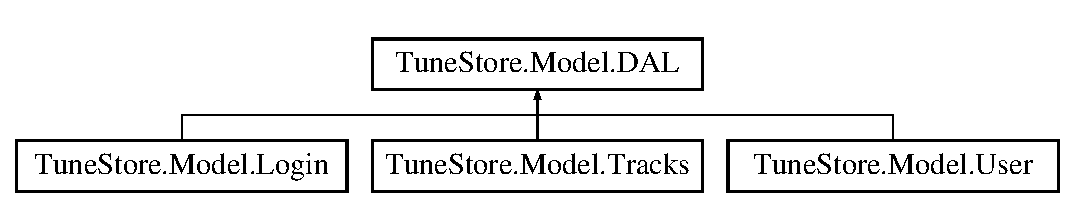
\includegraphics[height=2.000000cm]{class_tune_store_1_1_model_1_1_d_a_l}
\end{center}
\end{figure}
\subsection*{Static Public Member Functions}
\begin{DoxyCompactItemize}
\item 
static string \hyperlink{class_tune_store_1_1_model_1_1_d_a_l_abc0363548c4a5260b488da0180643388}{M\+D5\+Hash} (string text)
\begin{DoxyCompactList}\small\item\em String to M\+D5 hash generator \end{DoxyCompactList}\end{DoxyCompactItemize}
\subsection*{Protected Member Functions}
\begin{DoxyCompactItemize}
\item 
\hypertarget{class_tune_store_1_1_model_1_1_d_a_l_ac7f3fcd580550051af6d55ad6f60b4d6}{bool {\bfseries Is\+Connect\+Created} ()}\label{class_tune_store_1_1_model_1_1_d_a_l_ac7f3fcd580550051af6d55ad6f60b4d6}

\item 
\hypertarget{class_tune_store_1_1_model_1_1_d_a_l_afbed4e1710000cf02ff78502fc129e91}{bool {\bfseries Is\+Connected} ()}\label{class_tune_store_1_1_model_1_1_d_a_l_afbed4e1710000cf02ff78502fc129e91}

\item 
\hypertarget{class_tune_store_1_1_model_1_1_d_a_l_a95b31c4a1c14fda499a962abf81df3c5}{Sql\+Connection {\bfseries Get\+Connection} ()}\label{class_tune_store_1_1_model_1_1_d_a_l_a95b31c4a1c14fda499a962abf81df3c5}

\item 
bool \hyperlink{class_tune_store_1_1_model_1_1_d_a_l_ab31c1978d9d09f57793cf307807bc577}{Create\+Connection} ()
\begin{DoxyCompactList}\small\item\em Creates a new Database Connection \end{DoxyCompactList}\item 
bool \hyperlink{class_tune_store_1_1_model_1_1_d_a_l_a95012ed2fb7e4242eb95199315a86eaf}{Open\+Connection} ()
\begin{DoxyCompactList}\small\item\em Open the Connection when the state is not already open. \end{DoxyCompactList}\item 
object \hyperlink{class_tune_store_1_1_model_1_1_d_a_l_ad29e5842a6d4df190309dab55aaa6cb7}{Execute\+Scalar} (string query, ref string error\+Message)
\begin{DoxyCompactList}\small\item\em Execute sql query \end{DoxyCompactList}\item 
Sql\+Data\+Reader \hyperlink{class_tune_store_1_1_model_1_1_d_a_l_a084bc2866f85d34bdd6d4ece7f9472e3}{Execute\+Reader} (string query, ref string error\+Message)
\begin{DoxyCompactList}\small\item\em Executes a given query, and returns the result in a datareader \end{DoxyCompactList}\item 
void \hyperlink{class_tune_store_1_1_model_1_1_d_a_l_ac8f347f0d27aeadc61bc341276664290}{Close\+Data\+Reader} (Sql\+Data\+Reader rdr)
\begin{DoxyCompactList}\small\item\em Closes the data reader given as a parameter, and also closes the connection \end{DoxyCompactList}\item 
string \hyperlink{class_tune_store_1_1_model_1_1_d_a_l_a50bce22a6e2222ef51e1d79d1cb1da18}{Execute\+Non\+Query} (string command)
\begin{DoxyCompactList}\small\item\em Executes a given insert/update/delete command, and returns an error message. (errormessage is \char`\"{}\+O\+K\char`\"{} if no exception occured) \end{DoxyCompactList}\item 
string \hyperlink{class_tune_store_1_1_model_1_1_d_a_l_a2a16f122db8e86f86a8b21fffffec3ef}{Execute\+Stored\+Procedure\+Non\+Query} (string name, string\mbox{[}$\,$\mbox{]} parameter\+Names, string\mbox{[}$\,$\mbox{]} parameter\+Values)
\begin{DoxyCompactList}\small\item\em Executes a stored procedure that doesn't have any otuput parameters. \end{DoxyCompactList}\end{DoxyCompactItemize}
\subsection*{Protected Attributes}
\begin{DoxyCompactItemize}
\item 
\hypertarget{class_tune_store_1_1_model_1_1_d_a_l_a4966b46d96f1ef56313015457f72e7ca}{string {\bfseries m\+\_\+\+Connection\+String} = \char`\"{}Data Source=M\+A\+T\+T\+Y\+Y-\/P\+C;Initial Catalog=Tune\+Store;Integrated Security=S\+S\+P\+I\char`\"{}}\label{class_tune_store_1_1_model_1_1_d_a_l_a4966b46d96f1ef56313015457f72e7ca}

\item 
\hypertarget{class_tune_store_1_1_model_1_1_d_a_l_aae6028ff60c0a0103a096e870ce097d0}{Sql\+Command {\bfseries m\+\_\+\+Command}}\label{class_tune_store_1_1_model_1_1_d_a_l_aae6028ff60c0a0103a096e870ce097d0}

\end{DoxyCompactItemize}
\subsection*{Static Protected Attributes}
\begin{DoxyCompactItemize}
\item 
\hypertarget{class_tune_store_1_1_model_1_1_d_a_l_a10ca522dc93f490d832ef98c7770ed7b}{static bool {\bfseries Connected}}\label{class_tune_store_1_1_model_1_1_d_a_l_a10ca522dc93f490d832ef98c7770ed7b}

\item 
\hypertarget{class_tune_store_1_1_model_1_1_d_a_l_a185064dd52f541717750cd3de77b0ddd}{static bool {\bfseries Connection\+Created}}\label{class_tune_store_1_1_model_1_1_d_a_l_a185064dd52f541717750cd3de77b0ddd}

\item 
\hypertarget{class_tune_store_1_1_model_1_1_d_a_l_af14bf3278fe3c80fa06b315ed5e93523}{static Sql\+Connection {\bfseries m\+\_\+\+Connection}}\label{class_tune_store_1_1_model_1_1_d_a_l_af14bf3278fe3c80fa06b315ed5e93523}

\end{DoxyCompactItemize}


\subsection{Detailed Description}
Data access layer superclass of model classes 



Definition at line 17 of file D\+A\+L.\+cs.



\subsection{Member Function Documentation}
\hypertarget{class_tune_store_1_1_model_1_1_d_a_l_ac8f347f0d27aeadc61bc341276664290}{\index{Tune\+Store\+::\+Model\+::\+D\+A\+L@{Tune\+Store\+::\+Model\+::\+D\+A\+L}!Close\+Data\+Reader@{Close\+Data\+Reader}}
\index{Close\+Data\+Reader@{Close\+Data\+Reader}!Tune\+Store\+::\+Model\+::\+D\+A\+L@{Tune\+Store\+::\+Model\+::\+D\+A\+L}}
\subsubsection[{Close\+Data\+Reader}]{\setlength{\rightskip}{0pt plus 5cm}void Tune\+Store.\+Model.\+D\+A\+L.\+Close\+Data\+Reader (
\begin{DoxyParamCaption}
\item[{Sql\+Data\+Reader}]{rdr}
\end{DoxyParamCaption}
)\hspace{0.3cm}{\ttfamily [protected]}}}\label{class_tune_store_1_1_model_1_1_d_a_l_ac8f347f0d27aeadc61bc341276664290}


Closes the data reader given as a parameter, and also closes the connection 


\begin{DoxyParams}{Parameters}
{\em rdr} & The Sql\+Data\+Reader to be closed\\
\hline
\end{DoxyParams}


Definition at line 172 of file D\+A\+L.\+cs.

\hypertarget{class_tune_store_1_1_model_1_1_d_a_l_ab31c1978d9d09f57793cf307807bc577}{\index{Tune\+Store\+::\+Model\+::\+D\+A\+L@{Tune\+Store\+::\+Model\+::\+D\+A\+L}!Create\+Connection@{Create\+Connection}}
\index{Create\+Connection@{Create\+Connection}!Tune\+Store\+::\+Model\+::\+D\+A\+L@{Tune\+Store\+::\+Model\+::\+D\+A\+L}}
\subsubsection[{Create\+Connection}]{\setlength{\rightskip}{0pt plus 5cm}bool Tune\+Store.\+Model.\+D\+A\+L.\+Create\+Connection (
\begin{DoxyParamCaption}
{}
\end{DoxyParamCaption}
)\hspace{0.3cm}{\ttfamily [protected]}}}\label{class_tune_store_1_1_model_1_1_d_a_l_ab31c1978d9d09f57793cf307807bc577}


Creates a new Database Connection 

\begin{DoxyReturn}{Returns}

\end{DoxyReturn}


Definition at line 48 of file D\+A\+L.\+cs.

\hypertarget{class_tune_store_1_1_model_1_1_d_a_l_a50bce22a6e2222ef51e1d79d1cb1da18}{\index{Tune\+Store\+::\+Model\+::\+D\+A\+L@{Tune\+Store\+::\+Model\+::\+D\+A\+L}!Execute\+Non\+Query@{Execute\+Non\+Query}}
\index{Execute\+Non\+Query@{Execute\+Non\+Query}!Tune\+Store\+::\+Model\+::\+D\+A\+L@{Tune\+Store\+::\+Model\+::\+D\+A\+L}}
\subsubsection[{Execute\+Non\+Query}]{\setlength{\rightskip}{0pt plus 5cm}string Tune\+Store.\+Model.\+D\+A\+L.\+Execute\+Non\+Query (
\begin{DoxyParamCaption}
\item[{string}]{command}
\end{DoxyParamCaption}
)\hspace{0.3cm}{\ttfamily [protected]}}}\label{class_tune_store_1_1_model_1_1_d_a_l_a50bce22a6e2222ef51e1d79d1cb1da18}


Executes a given insert/update/delete command, and returns an error message. (errormessage is \char`\"{}\+O\+K\char`\"{} if no exception occured) 


\begin{DoxyParams}{Parameters}
{\em command} & The command to be executed\\
\hline
\end{DoxyParams}


Definition at line 184 of file D\+A\+L.\+cs.

\hypertarget{class_tune_store_1_1_model_1_1_d_a_l_a084bc2866f85d34bdd6d4ece7f9472e3}{\index{Tune\+Store\+::\+Model\+::\+D\+A\+L@{Tune\+Store\+::\+Model\+::\+D\+A\+L}!Execute\+Reader@{Execute\+Reader}}
\index{Execute\+Reader@{Execute\+Reader}!Tune\+Store\+::\+Model\+::\+D\+A\+L@{Tune\+Store\+::\+Model\+::\+D\+A\+L}}
\subsubsection[{Execute\+Reader}]{\setlength{\rightskip}{0pt plus 5cm}Sql\+Data\+Reader Tune\+Store.\+Model.\+D\+A\+L.\+Execute\+Reader (
\begin{DoxyParamCaption}
\item[{string}]{query, }
\item[{ref string}]{error\+Message}
\end{DoxyParamCaption}
)\hspace{0.3cm}{\ttfamily [protected]}}}\label{class_tune_store_1_1_model_1_1_d_a_l_a084bc2866f85d34bdd6d4ece7f9472e3}


Executes a given query, and returns the result in a datareader 


\begin{DoxyParams}{Parameters}
{\em query} & The query to be executed \\
\hline
{\em error\+Message} & Output error message \\
\hline
\end{DoxyParams}
\begin{DoxyReturn}{Returns}

\end{DoxyReturn}


Definition at line 149 of file D\+A\+L.\+cs.

\hypertarget{class_tune_store_1_1_model_1_1_d_a_l_ad29e5842a6d4df190309dab55aaa6cb7}{\index{Tune\+Store\+::\+Model\+::\+D\+A\+L@{Tune\+Store\+::\+Model\+::\+D\+A\+L}!Execute\+Scalar@{Execute\+Scalar}}
\index{Execute\+Scalar@{Execute\+Scalar}!Tune\+Store\+::\+Model\+::\+D\+A\+L@{Tune\+Store\+::\+Model\+::\+D\+A\+L}}
\subsubsection[{Execute\+Scalar}]{\setlength{\rightskip}{0pt plus 5cm}object Tune\+Store.\+Model.\+D\+A\+L.\+Execute\+Scalar (
\begin{DoxyParamCaption}
\item[{string}]{query, }
\item[{ref string}]{error\+Message}
\end{DoxyParamCaption}
)\hspace{0.3cm}{\ttfamily [protected]}}}\label{class_tune_store_1_1_model_1_1_d_a_l_ad29e5842a6d4df190309dab55aaa6cb7}


Execute sql query 


\begin{DoxyParams}{Parameters}
{\em query} & Query string\\
\hline
{\em error\+Message} & \\
\hline
\end{DoxyParams}
\begin{DoxyReturn}{Returns}

\end{DoxyReturn}


Definition at line 121 of file D\+A\+L.\+cs.

\hypertarget{class_tune_store_1_1_model_1_1_d_a_l_a2a16f122db8e86f86a8b21fffffec3ef}{\index{Tune\+Store\+::\+Model\+::\+D\+A\+L@{Tune\+Store\+::\+Model\+::\+D\+A\+L}!Execute\+Stored\+Procedure\+Non\+Query@{Execute\+Stored\+Procedure\+Non\+Query}}
\index{Execute\+Stored\+Procedure\+Non\+Query@{Execute\+Stored\+Procedure\+Non\+Query}!Tune\+Store\+::\+Model\+::\+D\+A\+L@{Tune\+Store\+::\+Model\+::\+D\+A\+L}}
\subsubsection[{Execute\+Stored\+Procedure\+Non\+Query}]{\setlength{\rightskip}{0pt plus 5cm}string Tune\+Store.\+Model.\+D\+A\+L.\+Execute\+Stored\+Procedure\+Non\+Query (
\begin{DoxyParamCaption}
\item[{string}]{name, }
\item[{string\mbox{[}$\,$\mbox{]}}]{parameter\+Names, }
\item[{string\mbox{[}$\,$\mbox{]}}]{parameter\+Values}
\end{DoxyParamCaption}
)\hspace{0.3cm}{\ttfamily [protected]}}}\label{class_tune_store_1_1_model_1_1_d_a_l_a2a16f122db8e86f86a8b21fffffec3ef}


Executes a stored procedure that doesn't have any otuput parameters. 


\begin{DoxyParams}{Parameters}
{\em name} & The name of the stored procedure\\
\hline
{\em parameter\+Names} & The list of the parameter names\\
\hline
{\em parameter\+Values} & The list of the parameter values\\
\hline
\end{DoxyParams}
\begin{DoxyReturn}{Returns}

\end{DoxyReturn}


Definition at line 213 of file D\+A\+L.\+cs.

\hypertarget{class_tune_store_1_1_model_1_1_d_a_l_abc0363548c4a5260b488da0180643388}{\index{Tune\+Store\+::\+Model\+::\+D\+A\+L@{Tune\+Store\+::\+Model\+::\+D\+A\+L}!M\+D5\+Hash@{M\+D5\+Hash}}
\index{M\+D5\+Hash@{M\+D5\+Hash}!Tune\+Store\+::\+Model\+::\+D\+A\+L@{Tune\+Store\+::\+Model\+::\+D\+A\+L}}
\subsubsection[{M\+D5\+Hash}]{\setlength{\rightskip}{0pt plus 5cm}static string Tune\+Store.\+Model.\+D\+A\+L.\+M\+D5\+Hash (
\begin{DoxyParamCaption}
\item[{string}]{text}
\end{DoxyParamCaption}
)\hspace{0.3cm}{\ttfamily [static]}}}\label{class_tune_store_1_1_model_1_1_d_a_l_abc0363548c4a5260b488da0180643388}


String to M\+D5 hash generator 


\begin{DoxyParams}{Parameters}
{\em text} & \\
\hline
\end{DoxyParams}
\begin{DoxyReturn}{Returns}

\end{DoxyReturn}


Definition at line 245 of file D\+A\+L.\+cs.

\hypertarget{class_tune_store_1_1_model_1_1_d_a_l_a95012ed2fb7e4242eb95199315a86eaf}{\index{Tune\+Store\+::\+Model\+::\+D\+A\+L@{Tune\+Store\+::\+Model\+::\+D\+A\+L}!Open\+Connection@{Open\+Connection}}
\index{Open\+Connection@{Open\+Connection}!Tune\+Store\+::\+Model\+::\+D\+A\+L@{Tune\+Store\+::\+Model\+::\+D\+A\+L}}
\subsubsection[{Open\+Connection}]{\setlength{\rightskip}{0pt plus 5cm}bool Tune\+Store.\+Model.\+D\+A\+L.\+Open\+Connection (
\begin{DoxyParamCaption}
{}
\end{DoxyParamCaption}
)\hspace{0.3cm}{\ttfamily [protected]}}}\label{class_tune_store_1_1_model_1_1_d_a_l_a95012ed2fb7e4242eb95199315a86eaf}


Open the Connection when the state is not already open. 



Definition at line 79 of file D\+A\+L.\+cs.



The documentation for this class was generated from the following file\+:\begin{DoxyCompactItemize}
\item 
Tune\+Store/\+Model/D\+A\+L.\+cs\end{DoxyCompactItemize}

\hypertarget{class_tune_store_1_1_model_1_1_login}{\section{Tune\+Store.\+Model.\+Login Class Reference}
\label{class_tune_store_1_1_model_1_1_login}\index{Tune\+Store.\+Model.\+Login@{Tune\+Store.\+Model.\+Login}}
}


\hyperlink{class_tune_store_1_1_model_1_1_user}{User} login on model layer  


Inheritance diagram for Tune\+Store.\+Model.\+Login\+:\begin{figure}[H]
\begin{center}
\leavevmode
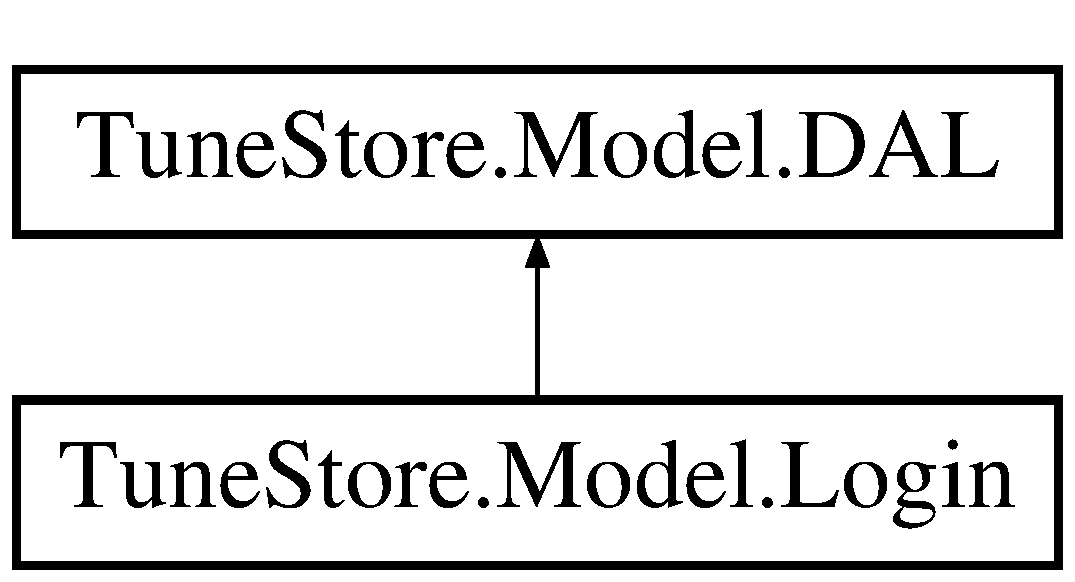
\includegraphics[height=2.000000cm]{class_tune_store_1_1_model_1_1_login}
\end{center}
\end{figure}
\subsection*{Public Member Functions}
\begin{DoxyCompactItemize}
\item 
\hyperlink{class_tune_store_1_1_model_1_1_login_a184a2123650754b3774309e52d535cc1}{Login} (string name, string pass)
\begin{DoxyCompactList}\small\item\em Constructor \end{DoxyCompactList}\end{DoxyCompactItemize}
\subsection*{Public Attributes}
\begin{DoxyCompactItemize}
\item 
\hypertarget{class_tune_store_1_1_model_1_1_login_aae18c7ab7670fa32ee078a0912fdd29e}{int {\bfseries user\+Id} = -\/1}\label{class_tune_store_1_1_model_1_1_login_aae18c7ab7670fa32ee078a0912fdd29e}

\item 
\hypertarget{class_tune_store_1_1_model_1_1_login_aebed49f7f6e757d809ec19ff90b27a8d}{String {\bfseries group} = \char`\"{}\char`\"{}}\label{class_tune_store_1_1_model_1_1_login_aebed49f7f6e757d809ec19ff90b27a8d}

\item 
\hypertarget{class_tune_store_1_1_model_1_1_login_a6cab707f0091ca10ed6e8493822d42f8}{String {\bfseries user\+Name} = \char`\"{}\char`\"{}}\label{class_tune_store_1_1_model_1_1_login_a6cab707f0091ca10ed6e8493822d42f8}

\item 
\hypertarget{class_tune_store_1_1_model_1_1_login_a3f9fb2ba7fda5853e9555673dc550c72}{bool {\bfseries logged\+In} = false}\label{class_tune_store_1_1_model_1_1_login_a3f9fb2ba7fda5853e9555673dc550c72}

\end{DoxyCompactItemize}
\subsection*{Additional Inherited Members}


\subsection{Detailed Description}
\hyperlink{class_tune_store_1_1_model_1_1_user}{User} login on model layer 



Definition at line 16 of file Login.\+cs.



\subsection{Constructor \& Destructor Documentation}
\hypertarget{class_tune_store_1_1_model_1_1_login_a184a2123650754b3774309e52d535cc1}{\index{Tune\+Store\+::\+Model\+::\+Login@{Tune\+Store\+::\+Model\+::\+Login}!Login@{Login}}
\index{Login@{Login}!Tune\+Store\+::\+Model\+::\+Login@{Tune\+Store\+::\+Model\+::\+Login}}
\subsubsection[{Login}]{\setlength{\rightskip}{0pt plus 5cm}Tune\+Store.\+Model.\+Login.\+Login (
\begin{DoxyParamCaption}
\item[{string}]{name, }
\item[{string}]{pass}
\end{DoxyParamCaption}
)}}\label{class_tune_store_1_1_model_1_1_login_a184a2123650754b3774309e52d535cc1}


Constructor 


\begin{DoxyParams}{Parameters}
{\em name} & Username\\
\hline
{\em pass} & Password\\
\hline
\end{DoxyParams}


Definition at line 28 of file Login.\+cs.



The documentation for this class was generated from the following file\+:\begin{DoxyCompactItemize}
\item 
Tune\+Store/\+Model/Login.\+cs\end{DoxyCompactItemize}

\hypertarget{class_tune_store_1_1_main_frame}{\section{Tune\+Store.\+Main\+Frame Class Reference}
\label{class_tune_store_1_1_main_frame}\index{Tune\+Store.\+Main\+Frame@{Tune\+Store.\+Main\+Frame}}
}


Main form, the view layer  


Inheritance diagram for Tune\+Store.\+Main\+Frame\+:\begin{figure}[H]
\begin{center}
\leavevmode
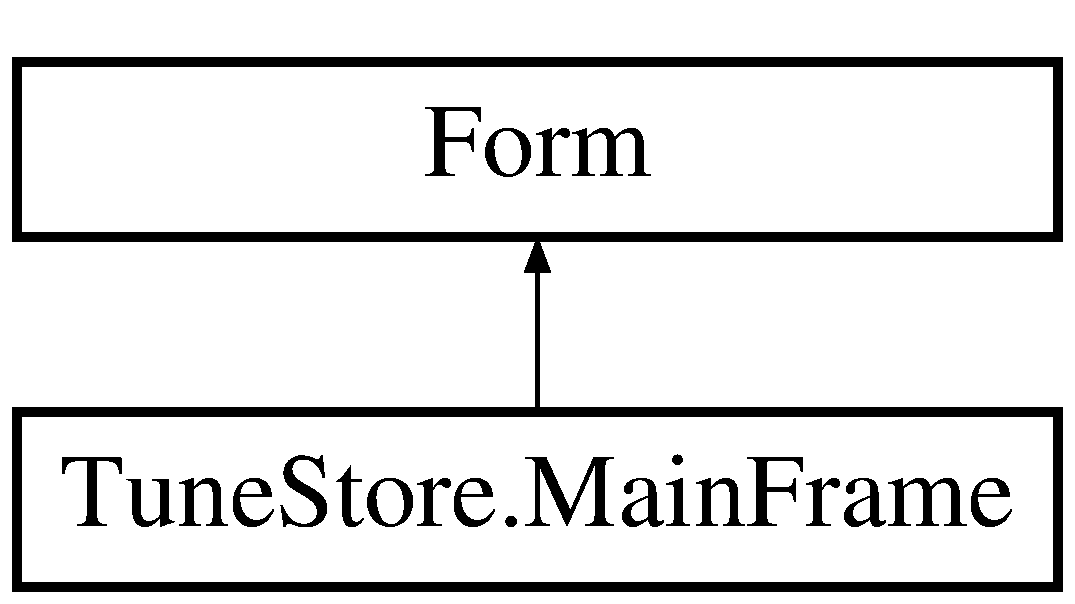
\includegraphics[height=2.000000cm]{class_tune_store_1_1_main_frame}
\end{center}
\end{figure}
\subsection*{Public Member Functions}
\begin{DoxyCompactItemize}
\item 
\hyperlink{class_tune_store_1_1_main_frame_ab0a7fd425cfbe4d9ed5351dbe0f0899a}{Main\+Frame} ()
\begin{DoxyCompactList}\small\item\em Main Frame constructor \end{DoxyCompactList}\item 
void \hyperlink{class_tune_store_1_1_main_frame_a8a32f6966fd90df24a85fadcea8ec7d1}{login\+Label\+\_\+\+Link\+Clicked} (object sender, Link\+Label\+Link\+Clicked\+Event\+Args e)
\begin{DoxyCompactList}\small\item\em Login event handler \end{DoxyCompactList}\item 
void \hyperlink{class_tune_store_1_1_main_frame_aaf0481f5c8f99cb447fc232ca5a698c1}{set\+View\+By\+User\+Type} (String utype)
\begin{DoxyCompactList}\small\item\em Setting view by user's group \end{DoxyCompactList}\item 
void \hyperlink{class_tune_store_1_1_main_frame_a919bb15a5b669920816a76924a5634c6}{set\+Info\+Labels} (Data\+Row trackinfo)
\begin{DoxyCompactList}\small\item\em Show track informations \end{DoxyCompactList}\item 
void \hyperlink{class_tune_store_1_1_main_frame_ab9e2975a8e69eef23679870fe908d373}{set\+Artwork\+Box} (Image i)
\begin{DoxyCompactList}\small\item\em Show artwork \end{DoxyCompactList}\end{DoxyCompactItemize}
\subsection*{Protected Member Functions}
\begin{DoxyCompactItemize}
\item 
override void \hyperlink{class_tune_store_1_1_main_frame_a6b8d40a788e25cf9904991e9b386746c}{Dispose} (bool disposing)
\begin{DoxyCompactList}\small\item\em Clean up any resources being used. \end{DoxyCompactList}\end{DoxyCompactItemize}
\subsection*{Properties}
\begin{DoxyCompactItemize}
\item 
\hypertarget{class_tune_store_1_1_main_frame_af8357e47c5adf1b4def03c2ef99ecb23}{\hyperlink{class_tune_store_1_1_runscriptfrm}{Runscriptfrm} {\bfseries Runscriptfrm}\hspace{0.3cm}{\ttfamily  \mbox{[}get, set\mbox{]}}}\label{class_tune_store_1_1_main_frame_af8357e47c5adf1b4def03c2ef99ecb23}

\end{DoxyCompactItemize}


\subsection{Detailed Description}
Main form, the view layer 



Definition at line 17 of file Tune\+Store.\+cs.



\subsection{Constructor \& Destructor Documentation}
\hypertarget{class_tune_store_1_1_main_frame_ab0a7fd425cfbe4d9ed5351dbe0f0899a}{\index{Tune\+Store\+::\+Main\+Frame@{Tune\+Store\+::\+Main\+Frame}!Main\+Frame@{Main\+Frame}}
\index{Main\+Frame@{Main\+Frame}!Tune\+Store\+::\+Main\+Frame@{Tune\+Store\+::\+Main\+Frame}}
\subsubsection[{Main\+Frame}]{\setlength{\rightskip}{0pt plus 5cm}Tune\+Store.\+Main\+Frame.\+Main\+Frame (
\begin{DoxyParamCaption}
{}
\end{DoxyParamCaption}
)}}\label{class_tune_store_1_1_main_frame_ab0a7fd425cfbe4d9ed5351dbe0f0899a}


Main Frame constructor 



Definition at line 28 of file Tune\+Store.\+cs.



\subsection{Member Function Documentation}
\hypertarget{class_tune_store_1_1_main_frame_a6b8d40a788e25cf9904991e9b386746c}{\index{Tune\+Store\+::\+Main\+Frame@{Tune\+Store\+::\+Main\+Frame}!Dispose@{Dispose}}
\index{Dispose@{Dispose}!Tune\+Store\+::\+Main\+Frame@{Tune\+Store\+::\+Main\+Frame}}
\subsubsection[{Dispose}]{\setlength{\rightskip}{0pt plus 5cm}override void Tune\+Store.\+Main\+Frame.\+Dispose (
\begin{DoxyParamCaption}
\item[{bool}]{disposing}
\end{DoxyParamCaption}
)\hspace{0.3cm}{\ttfamily [protected]}}}\label{class_tune_store_1_1_main_frame_a6b8d40a788e25cf9904991e9b386746c}


Clean up any resources being used. 


\begin{DoxyParams}{Parameters}
{\em disposing} & true if managed resources should be disposed; otherwise, false.\\
\hline
\end{DoxyParams}


Definition at line 14 of file Tune\+Store.\+Designer.\+cs.

\hypertarget{class_tune_store_1_1_main_frame_a8a32f6966fd90df24a85fadcea8ec7d1}{\index{Tune\+Store\+::\+Main\+Frame@{Tune\+Store\+::\+Main\+Frame}!login\+Label\+\_\+\+Link\+Clicked@{login\+Label\+\_\+\+Link\+Clicked}}
\index{login\+Label\+\_\+\+Link\+Clicked@{login\+Label\+\_\+\+Link\+Clicked}!Tune\+Store\+::\+Main\+Frame@{Tune\+Store\+::\+Main\+Frame}}
\subsubsection[{login\+Label\+\_\+\+Link\+Clicked}]{\setlength{\rightskip}{0pt plus 5cm}void Tune\+Store.\+Main\+Frame.\+login\+Label\+\_\+\+Link\+Clicked (
\begin{DoxyParamCaption}
\item[{object}]{sender, }
\item[{Link\+Label\+Link\+Clicked\+Event\+Args}]{e}
\end{DoxyParamCaption}
)}}\label{class_tune_store_1_1_main_frame_a8a32f6966fd90df24a85fadcea8ec7d1}


Login event handler 


\begin{DoxyParams}{Parameters}
{\em sender} & \\
\hline
{\em e} & \\
\hline
\end{DoxyParams}


Definition at line 208 of file Tune\+Store.\+cs.

\hypertarget{class_tune_store_1_1_main_frame_ab9e2975a8e69eef23679870fe908d373}{\index{Tune\+Store\+::\+Main\+Frame@{Tune\+Store\+::\+Main\+Frame}!set\+Artwork\+Box@{set\+Artwork\+Box}}
\index{set\+Artwork\+Box@{set\+Artwork\+Box}!Tune\+Store\+::\+Main\+Frame@{Tune\+Store\+::\+Main\+Frame}}
\subsubsection[{set\+Artwork\+Box}]{\setlength{\rightskip}{0pt plus 5cm}void Tune\+Store.\+Main\+Frame.\+set\+Artwork\+Box (
\begin{DoxyParamCaption}
\item[{Image}]{i}
\end{DoxyParamCaption}
)}}\label{class_tune_store_1_1_main_frame_ab9e2975a8e69eef23679870fe908d373}


Show artwork 


\begin{DoxyParams}{Parameters}
{\em i} & Artwork image \\
\hline
\end{DoxyParams}


Definition at line 486 of file Tune\+Store.\+cs.

\hypertarget{class_tune_store_1_1_main_frame_a919bb15a5b669920816a76924a5634c6}{\index{Tune\+Store\+::\+Main\+Frame@{Tune\+Store\+::\+Main\+Frame}!set\+Info\+Labels@{set\+Info\+Labels}}
\index{set\+Info\+Labels@{set\+Info\+Labels}!Tune\+Store\+::\+Main\+Frame@{Tune\+Store\+::\+Main\+Frame}}
\subsubsection[{set\+Info\+Labels}]{\setlength{\rightskip}{0pt plus 5cm}void Tune\+Store.\+Main\+Frame.\+set\+Info\+Labels (
\begin{DoxyParamCaption}
\item[{Data\+Row}]{trackinfo}
\end{DoxyParamCaption}
)}}\label{class_tune_store_1_1_main_frame_a919bb15a5b669920816a76924a5634c6}


Show track informations 


\begin{DoxyParams}{Parameters}
{\em trackinfo} & \\
\hline
\end{DoxyParams}


Definition at line 462 of file Tune\+Store.\+cs.

\hypertarget{class_tune_store_1_1_main_frame_aaf0481f5c8f99cb447fc232ca5a698c1}{\index{Tune\+Store\+::\+Main\+Frame@{Tune\+Store\+::\+Main\+Frame}!set\+View\+By\+User\+Type@{set\+View\+By\+User\+Type}}
\index{set\+View\+By\+User\+Type@{set\+View\+By\+User\+Type}!Tune\+Store\+::\+Main\+Frame@{Tune\+Store\+::\+Main\+Frame}}
\subsubsection[{set\+View\+By\+User\+Type}]{\setlength{\rightskip}{0pt plus 5cm}void Tune\+Store.\+Main\+Frame.\+set\+View\+By\+User\+Type (
\begin{DoxyParamCaption}
\item[{String}]{utype}
\end{DoxyParamCaption}
)}}\label{class_tune_store_1_1_main_frame_aaf0481f5c8f99cb447fc232ca5a698c1}


Setting view by user's group 


\begin{DoxyParams}{Parameters}
{\em utype} & User type\\
\hline
\end{DoxyParams}


Definition at line 334 of file Tune\+Store.\+cs.



The documentation for this class was generated from the following files\+:\begin{DoxyCompactItemize}
\item 
Tune\+Store/Tune\+Store.\+cs\item 
Tune\+Store/Tune\+Store.\+Designer.\+cs\end{DoxyCompactItemize}

\hypertarget{class_tune_store_1_1_runscriptfrm}{\section{Tune\+Store.\+Runscriptfrm Class Reference}
\label{class_tune_store_1_1_runscriptfrm}\index{Tune\+Store.\+Runscriptfrm@{Tune\+Store.\+Runscriptfrm}}
}


A form for running a given script, shows the console and the error output.  


Inheritance diagram for Tune\+Store.\+Runscriptfrm\+:\begin{figure}[H]
\begin{center}
\leavevmode
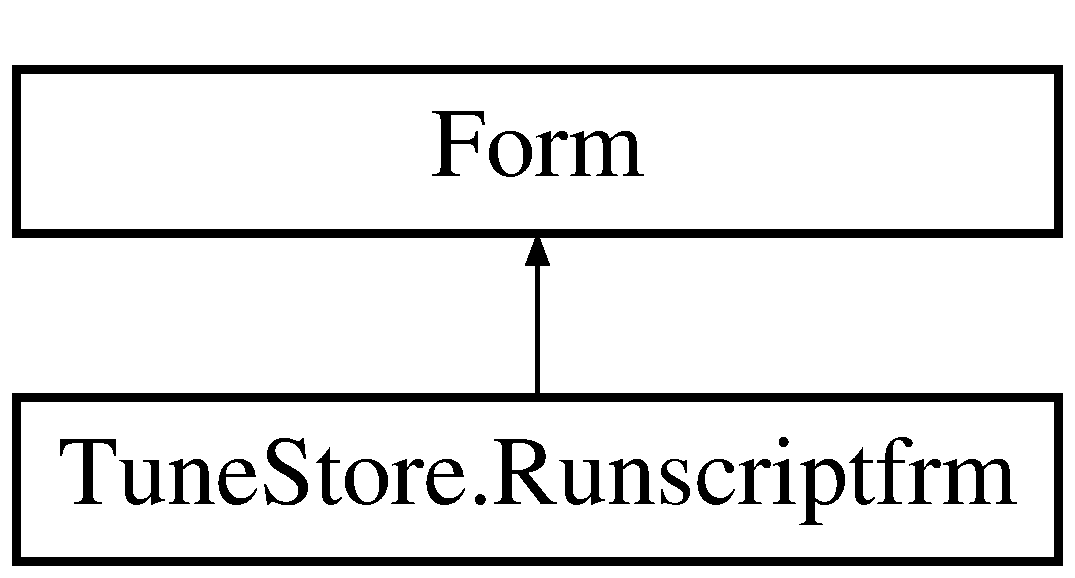
\includegraphics[height=2.000000cm]{class_tune_store_1_1_runscriptfrm}
\end{center}
\end{figure}
\subsection*{Public Member Functions}
\begin{DoxyCompactItemize}
\item 
\hyperlink{class_tune_store_1_1_runscriptfrm_a8a5c24209522b82788714f4716c7c546}{Runscriptfrm} (string script)
\begin{DoxyCompactList}\small\item\em Constructor \end{DoxyCompactList}\end{DoxyCompactItemize}
\subsection*{Protected Member Functions}
\begin{DoxyCompactItemize}
\item 
override void \hyperlink{class_tune_store_1_1_runscriptfrm_a6ddba7aa56bf04fba48a4239a78831dc}{Dispose} (bool disposing)
\begin{DoxyCompactList}\small\item\em Clean up any resources being used. \end{DoxyCompactList}\end{DoxyCompactItemize}


\subsection{Detailed Description}
A form for running a given script, shows the console and the error output. 



Definition at line 18 of file Runscriptfrm.\+cs.



\subsection{Constructor \& Destructor Documentation}
\hypertarget{class_tune_store_1_1_runscriptfrm_a8a5c24209522b82788714f4716c7c546}{\index{Tune\+Store\+::\+Runscriptfrm@{Tune\+Store\+::\+Runscriptfrm}!Runscriptfrm@{Runscriptfrm}}
\index{Runscriptfrm@{Runscriptfrm}!Tune\+Store\+::\+Runscriptfrm@{Tune\+Store\+::\+Runscriptfrm}}
\subsubsection[{Runscriptfrm}]{\setlength{\rightskip}{0pt plus 5cm}Tune\+Store.\+Runscriptfrm.\+Runscriptfrm (
\begin{DoxyParamCaption}
\item[{string}]{script}
\end{DoxyParamCaption}
)}}\label{class_tune_store_1_1_runscriptfrm_a8a5c24209522b82788714f4716c7c546}


Constructor 


\begin{DoxyParams}{Parameters}
{\em script} & String to script path\\
\hline
\end{DoxyParams}


Definition at line 28 of file Runscriptfrm.\+cs.



\subsection{Member Function Documentation}
\hypertarget{class_tune_store_1_1_runscriptfrm_a6ddba7aa56bf04fba48a4239a78831dc}{\index{Tune\+Store\+::\+Runscriptfrm@{Tune\+Store\+::\+Runscriptfrm}!Dispose@{Dispose}}
\index{Dispose@{Dispose}!Tune\+Store\+::\+Runscriptfrm@{Tune\+Store\+::\+Runscriptfrm}}
\subsubsection[{Dispose}]{\setlength{\rightskip}{0pt plus 5cm}override void Tune\+Store.\+Runscriptfrm.\+Dispose (
\begin{DoxyParamCaption}
\item[{bool}]{disposing}
\end{DoxyParamCaption}
)\hspace{0.3cm}{\ttfamily [protected]}}}\label{class_tune_store_1_1_runscriptfrm_a6ddba7aa56bf04fba48a4239a78831dc}


Clean up any resources being used. 


\begin{DoxyParams}{Parameters}
{\em disposing} & true if managed resources should be disposed; otherwise, false.\\
\hline
\end{DoxyParams}


Definition at line 14 of file Runscriptfrm.\+Designer.\+cs.



The documentation for this class was generated from the following files\+:\begin{DoxyCompactItemize}
\item 
Tune\+Store/Runscriptfrm.\+cs\item 
Tune\+Store/Runscriptfrm.\+Designer.\+cs\end{DoxyCompactItemize}

\hypertarget{class_tune_store_1_1_model_1_1_tracks}{\section{Tune\+Store.\+Model.\+Tracks Class Reference}
\label{class_tune_store_1_1_model_1_1_tracks}\index{Tune\+Store.\+Model.\+Tracks@{Tune\+Store.\+Model.\+Tracks}}
}


\hyperlink{class_tune_store_1_1_model_1_1_tracks}{Tracks} access layer  


Inheritance diagram for Tune\+Store.\+Model.\+Tracks\+:\begin{figure}[H]
\begin{center}
\leavevmode
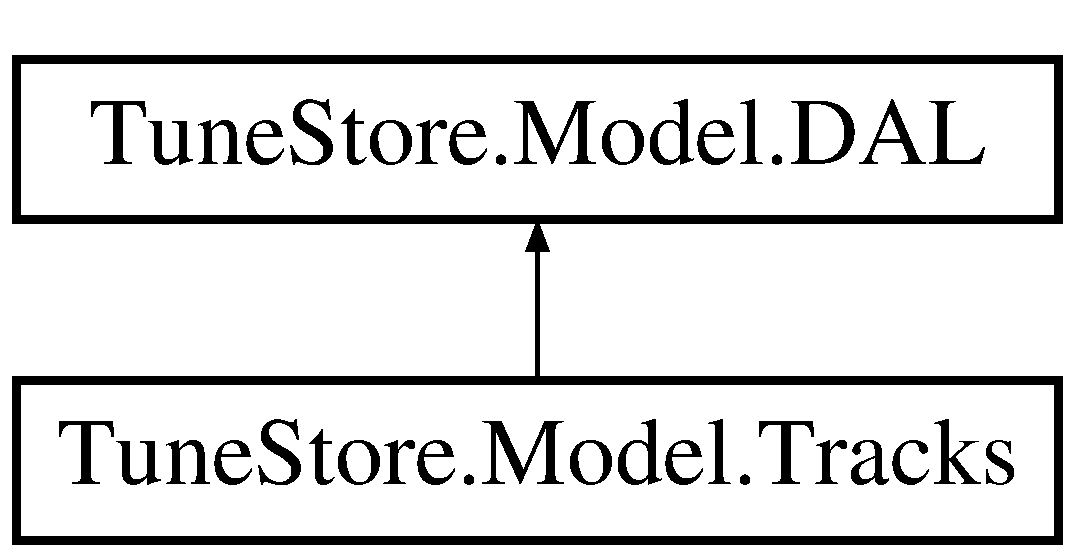
\includegraphics[height=2.000000cm]{class_tune_store_1_1_model_1_1_tracks}
\end{center}
\end{figure}
\subsection*{Public Member Functions}
\begin{DoxyCompactItemize}
\item 
\hyperlink{class_tune_store_1_1_model_1_1_tracks_ac5ca23ca4329b7a9f060d6307275e052}{Tracks} (int Id)
\begin{DoxyCompactList}\small\item\em Constructor \end{DoxyCompactList}\item 
Data\+Table \hyperlink{class_tune_store_1_1_model_1_1_tracks_ab86f9768aa3f019fde99e3545c1fc5b2}{get\+Data\+Table} (String query)
\begin{DoxyCompactList}\small\item\em Get a Data\+Table from given query \end{DoxyCompactList}\end{DoxyCompactItemize}
\subsection*{Static Public Member Functions}
\begin{DoxyCompactItemize}
\item 
static string \hyperlink{class_tune_store_1_1_model_1_1_tracks_a99770d353dc98772b4d24a7eaf90c831}{get\+Filter\+String} (string artist, string album, string title, string genre, string key)
\begin{DoxyCompactList}\small\item\em Get query string from given filtering parameters \end{DoxyCompactList}\end{DoxyCompactItemize}
\subsection*{Additional Inherited Members}


\subsection{Detailed Description}
\hyperlink{class_tune_store_1_1_model_1_1_tracks}{Tracks} access layer 



Definition at line 17 of file Tracks.\+cs.



\subsection{Constructor \& Destructor Documentation}
\hypertarget{class_tune_store_1_1_model_1_1_tracks_ac5ca23ca4329b7a9f060d6307275e052}{\index{Tune\+Store\+::\+Model\+::\+Tracks@{Tune\+Store\+::\+Model\+::\+Tracks}!Tracks@{Tracks}}
\index{Tracks@{Tracks}!Tune\+Store\+::\+Model\+::\+Tracks@{Tune\+Store\+::\+Model\+::\+Tracks}}
\subsubsection[{Tracks}]{\setlength{\rightskip}{0pt plus 5cm}Tune\+Store.\+Model.\+Tracks.\+Tracks (
\begin{DoxyParamCaption}
\item[{int}]{Id}
\end{DoxyParamCaption}
)}}\label{class_tune_store_1_1_model_1_1_tracks_ac5ca23ca4329b7a9f060d6307275e052}


Constructor 


\begin{DoxyParams}{Parameters}
{\em Id} & \hyperlink{class_tune_store_1_1_model_1_1_user}{User} identifier\\
\hline
\end{DoxyParams}


Definition at line 25 of file Tracks.\+cs.



\subsection{Member Function Documentation}
\hypertarget{class_tune_store_1_1_model_1_1_tracks_ab86f9768aa3f019fde99e3545c1fc5b2}{\index{Tune\+Store\+::\+Model\+::\+Tracks@{Tune\+Store\+::\+Model\+::\+Tracks}!get\+Data\+Table@{get\+Data\+Table}}
\index{get\+Data\+Table@{get\+Data\+Table}!Tune\+Store\+::\+Model\+::\+Tracks@{Tune\+Store\+::\+Model\+::\+Tracks}}
\subsubsection[{get\+Data\+Table}]{\setlength{\rightskip}{0pt plus 5cm}Data\+Table Tune\+Store.\+Model.\+Tracks.\+get\+Data\+Table (
\begin{DoxyParamCaption}
\item[{String}]{query}
\end{DoxyParamCaption}
)}}\label{class_tune_store_1_1_model_1_1_tracks_ab86f9768aa3f019fde99e3545c1fc5b2}


Get a Data\+Table from given query 


\begin{DoxyParams}{Parameters}
{\em query} & \\
\hline
\end{DoxyParams}
\begin{DoxyReturn}{Returns}
Data\+Table with requested tracks
\end{DoxyReturn}


Definition at line 35 of file Tracks.\+cs.

\hypertarget{class_tune_store_1_1_model_1_1_tracks_a99770d353dc98772b4d24a7eaf90c831}{\index{Tune\+Store\+::\+Model\+::\+Tracks@{Tune\+Store\+::\+Model\+::\+Tracks}!get\+Filter\+String@{get\+Filter\+String}}
\index{get\+Filter\+String@{get\+Filter\+String}!Tune\+Store\+::\+Model\+::\+Tracks@{Tune\+Store\+::\+Model\+::\+Tracks}}
\subsubsection[{get\+Filter\+String}]{\setlength{\rightskip}{0pt plus 5cm}static string Tune\+Store.\+Model.\+Tracks.\+get\+Filter\+String (
\begin{DoxyParamCaption}
\item[{string}]{artist, }
\item[{string}]{album, }
\item[{string}]{title, }
\item[{string}]{genre, }
\item[{string}]{key}
\end{DoxyParamCaption}
)\hspace{0.3cm}{\ttfamily [static]}}}\label{class_tune_store_1_1_model_1_1_tracks_a99770d353dc98772b4d24a7eaf90c831}


Get query string from given filtering parameters 


\begin{DoxyParams}{Parameters}
{\em artist} & Artist Name\\
\hline
{\em album} & Album Title\\
\hline
{\em title} & Track Title\\
\hline
{\em genre} & Genre name\\
\hline
{\em key} & Key\\
\hline
\end{DoxyParams}
\begin{DoxyReturn}{Returns}
Sql query string
\end{DoxyReturn}


Definition at line 70 of file Tracks.\+cs.



The documentation for this class was generated from the following file\+:\begin{DoxyCompactItemize}
\item 
Tune\+Store/\+Model/Tracks.\+cs\end{DoxyCompactItemize}

\hypertarget{class_tune_store_1_1_controller_1_1_tracks_controller}{\section{Tune\+Store.\+Controller.\+Tracks\+Controller Class Reference}
\label{class_tune_store_1_1_controller_1_1_tracks_controller}\index{Tune\+Store.\+Controller.\+Tracks\+Controller@{Tune\+Store.\+Controller.\+Tracks\+Controller}}
}


Track operations controller  


\subsection*{Public Member Functions}
\begin{DoxyCompactItemize}
\item 
\hyperlink{class_tune_store_1_1_controller_1_1_tracks_controller_aeefb43f2ed0910ff16b03c2668550ec3}{Tracks\+Controller} (\hyperlink{class_tune_store_1_1_main_frame}{Main\+Frame} mf, \hyperlink{class_tune_store_1_1_controller_1_1_user_controller}{User\+Controller} uc)
\begin{DoxyCompactList}\small\item\em Class constructor \end{DoxyCompactList}\end{DoxyCompactItemize}


\subsection{Detailed Description}
Track operations controller 



Definition at line 16 of file Tracks\+Controller.\+cs.



\subsection{Constructor \& Destructor Documentation}
\hypertarget{class_tune_store_1_1_controller_1_1_tracks_controller_aeefb43f2ed0910ff16b03c2668550ec3}{\index{Tune\+Store\+::\+Controller\+::\+Tracks\+Controller@{Tune\+Store\+::\+Controller\+::\+Tracks\+Controller}!Tracks\+Controller@{Tracks\+Controller}}
\index{Tracks\+Controller@{Tracks\+Controller}!Tune\+Store\+::\+Controller\+::\+Tracks\+Controller@{Tune\+Store\+::\+Controller\+::\+Tracks\+Controller}}
\subsubsection[{Tracks\+Controller}]{\setlength{\rightskip}{0pt plus 5cm}Tune\+Store.\+Controller.\+Tracks\+Controller.\+Tracks\+Controller (
\begin{DoxyParamCaption}
\item[{{\bf Main\+Frame}}]{mf, }
\item[{{\bf User\+Controller}}]{uc}
\end{DoxyParamCaption}
)}}\label{class_tune_store_1_1_controller_1_1_tracks_controller_aeefb43f2ed0910ff16b03c2668550ec3}


Class constructor 


\begin{DoxyParams}{Parameters}
{\em mf} & View form\\
\hline
{\em uc} & \hyperlink{namespace_tune_store_1_1_controller}{Controller} for logged in user\\
\hline
\end{DoxyParams}


Definition at line 28 of file Tracks\+Controller.\+cs.



The documentation for this class was generated from the following file\+:\begin{DoxyCompactItemize}
\item 
Tune\+Store/\+Controller/Tracks\+Controller.\+cs\end{DoxyCompactItemize}

\hypertarget{class_tune_store_1_1_model_1_1_user}{\section{Tune\+Store.\+Model.\+User Class Reference}
\label{class_tune_store_1_1_model_1_1_user}\index{Tune\+Store.\+Model.\+User@{Tune\+Store.\+Model.\+User}}
}


\hyperlink{class_tune_store_1_1_model_1_1_user}{User} registration into database,user information modifying  


Inheritance diagram for Tune\+Store.\+Model.\+User\+:\begin{figure}[H]
\begin{center}
\leavevmode
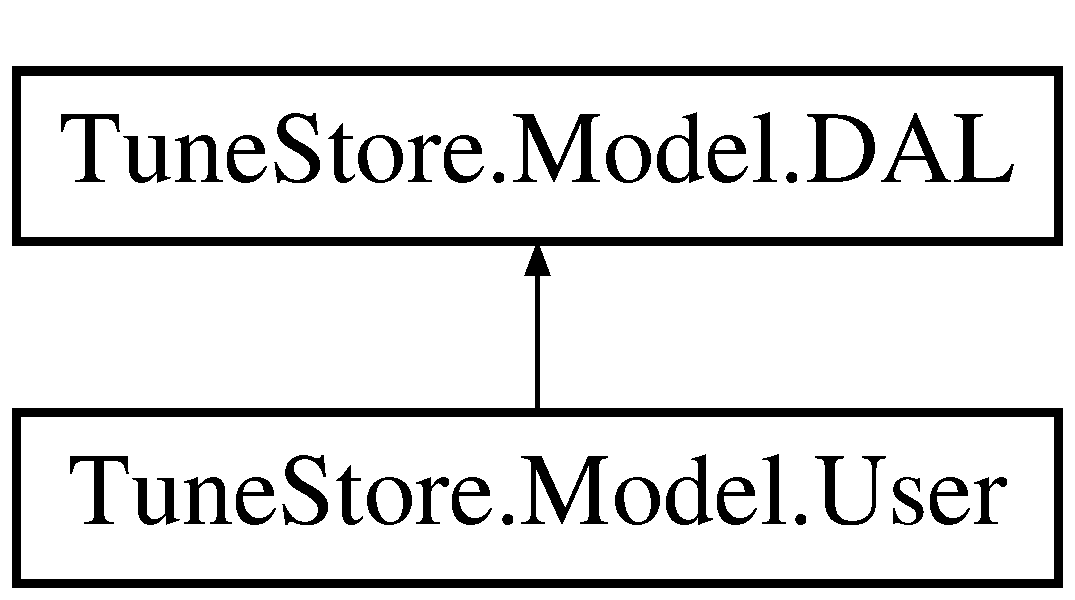
\includegraphics[height=2.000000cm]{class_tune_store_1_1_model_1_1_user}
\end{center}
\end{figure}
\subsection*{Public Member Functions}
\begin{DoxyCompactItemize}
\item 
\hyperlink{class_tune_store_1_1_model_1_1_user_a1fe1df691a5d73e5cd002f95493507c6}{User} (int u\+I\+D)
\begin{DoxyCompactList}\small\item\em Constructor \end{DoxyCompactList}\end{DoxyCompactItemize}
\subsection*{Static Public Member Functions}
\begin{DoxyCompactItemize}
\item 
static bool \hyperlink{class_tune_store_1_1_model_1_1_user_a20b4b1fd62760b59ac9a12f6b023e048}{register\+User} (Dictionary$<$ String, String $>$ regval)
\begin{DoxyCompactList}\small\item\em Register user \end{DoxyCompactList}\end{DoxyCompactItemize}
\subsection*{Public Attributes}
\begin{DoxyCompactItemize}
\item 
\hypertarget{class_tune_store_1_1_model_1_1_user_a123ef03d0c579697ed6be60d6dfb9e8a}{int {\bfseries user\+I\+D}}\label{class_tune_store_1_1_model_1_1_user_a123ef03d0c579697ed6be60d6dfb9e8a}

\item 
\hypertarget{class_tune_store_1_1_model_1_1_user_a3b6d61ac0f8fb592fa2ba08755e3f449}{String {\bfseries err} = \char`\"{}\char`\"{}}\label{class_tune_store_1_1_model_1_1_user_a3b6d61ac0f8fb592fa2ba08755e3f449}

\end{DoxyCompactItemize}
\subsection*{Additional Inherited Members}


\subsection{Detailed Description}
\hyperlink{class_tune_store_1_1_model_1_1_user}{User} registration into database,user information modifying 



Definition at line 15 of file User.\+cs.



\subsection{Constructor \& Destructor Documentation}
\hypertarget{class_tune_store_1_1_model_1_1_user_a1fe1df691a5d73e5cd002f95493507c6}{\index{Tune\+Store\+::\+Model\+::\+User@{Tune\+Store\+::\+Model\+::\+User}!User@{User}}
\index{User@{User}!Tune\+Store\+::\+Model\+::\+User@{Tune\+Store\+::\+Model\+::\+User}}
\subsubsection[{User}]{\setlength{\rightskip}{0pt plus 5cm}Tune\+Store.\+Model.\+User.\+User (
\begin{DoxyParamCaption}
\item[{int}]{u\+I\+D}
\end{DoxyParamCaption}
)}}\label{class_tune_store_1_1_model_1_1_user_a1fe1df691a5d73e5cd002f95493507c6}


Constructor 


\begin{DoxyParams}{Parameters}
{\em u\+I\+D} & User\+I\+D\\
\hline
\end{DoxyParams}


Definition at line 24 of file User.\+cs.



\subsection{Member Function Documentation}
\hypertarget{class_tune_store_1_1_model_1_1_user_a20b4b1fd62760b59ac9a12f6b023e048}{\index{Tune\+Store\+::\+Model\+::\+User@{Tune\+Store\+::\+Model\+::\+User}!register\+User@{register\+User}}
\index{register\+User@{register\+User}!Tune\+Store\+::\+Model\+::\+User@{Tune\+Store\+::\+Model\+::\+User}}
\subsubsection[{register\+User}]{\setlength{\rightskip}{0pt plus 5cm}static bool Tune\+Store.\+Model.\+User.\+register\+User (
\begin{DoxyParamCaption}
\item[{Dictionary$<$ String, String $>$}]{regval}
\end{DoxyParamCaption}
)\hspace{0.3cm}{\ttfamily [static]}}}\label{class_tune_store_1_1_model_1_1_user_a20b4b1fd62760b59ac9a12f6b023e048}


Register user 


\begin{DoxyParams}{Parameters}
{\em regval} & Dictionary containing Fieldname-\/\+Value\\
\hline
\end{DoxyParams}
\begin{DoxyReturn}{Returns}
Successful/\+Unsuccessful registration
\end{DoxyReturn}


Definition at line 34 of file User.\+cs.



The documentation for this class was generated from the following file\+:\begin{DoxyCompactItemize}
\item 
Tune\+Store/\+Model/User.\+cs\end{DoxyCompactItemize}

\hypertarget{class_tune_store_1_1_controller_1_1_user_controller}{\section{Tune\+Store.\+Controller.\+User\+Controller Class Reference}
\label{class_tune_store_1_1_controller_1_1_user_controller}\index{Tune\+Store.\+Controller.\+User\+Controller@{Tune\+Store.\+Controller.\+User\+Controller}}
}


\hyperlink{namespace_tune_store_1_1_controller}{Controller} class for user operations,  


\subsection*{Public Member Functions}
\begin{DoxyCompactItemize}
\item 
\hyperlink{class_tune_store_1_1_controller_1_1_user_controller_aedacc5c50043fe95376b9fbe548f1179}{User\+Controller} (\hyperlink{class_tune_store_1_1_main_frame}{Main\+Frame} ts)
\begin{DoxyCompactList}\small\item\em Guest user controller constructor \end{DoxyCompactList}\item 
Boolean \hyperlink{class_tune_store_1_1_controller_1_1_user_controller_aef029b55fd2db0e17720b06655bc34a1}{login} (String uname, String passw)
\begin{DoxyCompactList}\small\item\em Login user by username and password and set view by user type \end{DoxyCompactList}\item 
Boolean \hyperlink{class_tune_store_1_1_controller_1_1_user_controller_afa03d496d2db85b6da0017e9bb7a3b17}{logout} ()
\begin{DoxyCompactList}\small\item\em Logout user , set guest view \end{DoxyCompactList}\item 
int \hyperlink{class_tune_store_1_1_controller_1_1_user_controller_a6d842efdc09869eb99b577ed301e2bb2}{get\+User\+Id} ()
\begin{DoxyCompactList}\small\item\em User identifier(id) getter \end{DoxyCompactList}\end{DoxyCompactItemize}


\subsection{Detailed Description}
\hyperlink{namespace_tune_store_1_1_controller}{Controller} class for user operations, 



Definition at line 14 of file User\+Controller.\+cs.



\subsection{Constructor \& Destructor Documentation}
\hypertarget{class_tune_store_1_1_controller_1_1_user_controller_aedacc5c50043fe95376b9fbe548f1179}{\index{Tune\+Store\+::\+Controller\+::\+User\+Controller@{Tune\+Store\+::\+Controller\+::\+User\+Controller}!User\+Controller@{User\+Controller}}
\index{User\+Controller@{User\+Controller}!Tune\+Store\+::\+Controller\+::\+User\+Controller@{Tune\+Store\+::\+Controller\+::\+User\+Controller}}
\subsubsection[{User\+Controller}]{\setlength{\rightskip}{0pt plus 5cm}Tune\+Store.\+Controller.\+User\+Controller.\+User\+Controller (
\begin{DoxyParamCaption}
\item[{{\bf Main\+Frame}}]{ts}
\end{DoxyParamCaption}
)}}\label{class_tune_store_1_1_controller_1_1_user_controller_aedacc5c50043fe95376b9fbe548f1179}


Guest user controller constructor 


\begin{DoxyParams}{Parameters}
{\em ts} & View frame\\
\hline
\end{DoxyParams}


Definition at line 24 of file User\+Controller.\+cs.



\subsection{Member Function Documentation}
\hypertarget{class_tune_store_1_1_controller_1_1_user_controller_a6d842efdc09869eb99b577ed301e2bb2}{\index{Tune\+Store\+::\+Controller\+::\+User\+Controller@{Tune\+Store\+::\+Controller\+::\+User\+Controller}!get\+User\+Id@{get\+User\+Id}}
\index{get\+User\+Id@{get\+User\+Id}!Tune\+Store\+::\+Controller\+::\+User\+Controller@{Tune\+Store\+::\+Controller\+::\+User\+Controller}}
\subsubsection[{get\+User\+Id}]{\setlength{\rightskip}{0pt plus 5cm}int Tune\+Store.\+Controller.\+User\+Controller.\+get\+User\+Id (
\begin{DoxyParamCaption}
{}
\end{DoxyParamCaption}
)}}\label{class_tune_store_1_1_controller_1_1_user_controller_a6d842efdc09869eb99b577ed301e2bb2}


User identifier(id) getter 

\begin{DoxyReturn}{Returns}
User identifier(\+Int)
\end{DoxyReturn}


Definition at line 98 of file User\+Controller.\+cs.

\hypertarget{class_tune_store_1_1_controller_1_1_user_controller_aef029b55fd2db0e17720b06655bc34a1}{\index{Tune\+Store\+::\+Controller\+::\+User\+Controller@{Tune\+Store\+::\+Controller\+::\+User\+Controller}!login@{login}}
\index{login@{login}!Tune\+Store\+::\+Controller\+::\+User\+Controller@{Tune\+Store\+::\+Controller\+::\+User\+Controller}}
\subsubsection[{login}]{\setlength{\rightskip}{0pt plus 5cm}Boolean Tune\+Store.\+Controller.\+User\+Controller.\+login (
\begin{DoxyParamCaption}
\item[{String}]{uname, }
\item[{String}]{passw}
\end{DoxyParamCaption}
)}}\label{class_tune_store_1_1_controller_1_1_user_controller_aef029b55fd2db0e17720b06655bc34a1}


Login user by username and password and set view by user type 


\begin{DoxyParams}{Parameters}
{\em uname} & Username\\
\hline
{\em passw} & Password\\
\hline
\end{DoxyParams}
\begin{DoxyReturn}{Returns}
Succesful/\+Unsuccesful(true/false)
\end{DoxyReturn}


Definition at line 35 of file User\+Controller.\+cs.

\hypertarget{class_tune_store_1_1_controller_1_1_user_controller_afa03d496d2db85b6da0017e9bb7a3b17}{\index{Tune\+Store\+::\+Controller\+::\+User\+Controller@{Tune\+Store\+::\+Controller\+::\+User\+Controller}!logout@{logout}}
\index{logout@{logout}!Tune\+Store\+::\+Controller\+::\+User\+Controller@{Tune\+Store\+::\+Controller\+::\+User\+Controller}}
\subsubsection[{logout}]{\setlength{\rightskip}{0pt plus 5cm}Boolean Tune\+Store.\+Controller.\+User\+Controller.\+logout (
\begin{DoxyParamCaption}
{}
\end{DoxyParamCaption}
)}}\label{class_tune_store_1_1_controller_1_1_user_controller_afa03d496d2db85b6da0017e9bb7a3b17}


Logout user , set guest view 

\begin{DoxyReturn}{Returns}
True
\end{DoxyReturn}


Definition at line 49 of file User\+Controller.\+cs.



The documentation for this class was generated from the following file\+:\begin{DoxyCompactItemize}
\item 
Tune\+Store/\+Controller/User\+Controller.\+cs\end{DoxyCompactItemize}

%--- End generated contents ---

% Index
\newpage
\phantomsection
\addcontentsline{toc}{chapter}{Index}
\printindex

\end{document}
